% !TEX root = ../thesis.tex

\chapter{Evaluation} \label{evaluation}
Lets prepare the~experiment to validating a~long-term linear prediction model for online store orders.
We will use experimentation by these steps:\\
\begin{enumerate}
    \item Define the~problem and objectives: Clearly define the~problem and objectives that the~long-term linear
    prediction model is intended to solve. In this case, the~objective is to predict online store orders over a~long
    period of time using a~linear model.
    \item Gather data: Collect historical data on online store orders, such as order dates, order amounts, and other
    relevant variables. This data will be used to train and validate the~long-term linear prediction model.
    Our data was collect from online system storePredictor which is available on storepredictor.com and data are
    anonymized and pseudonimized to be used for next calculations.
    \item Prepare the~data: Clean and preprocess the~data to ensure that it is consistent and suitable for
    use in the~long-term linear prediction model. This may involve tasks such as removing duplicates, handling missing
    values, and transforming variables as needed. Preprocessing of our data is described in \ref{subsec:preprocessing}
    \item Develop the~long-term linear prediction model: Using the~historical data, develop a~long-term linear
    prediction model that can forecast online store orders over a~specified time period, which is detailed
    described in~\ref{sec:extlonglp} and practically applied in~\ref{subsec:calculate_models}
    over a~specified time period, described in~\ref{evaluation}.
    \item Evaluate the~results: Analyze the~results of the~experiment to determine the~accuracy of the~long-term
    linear prediction model. This will involve calculating metrics such as the~mean square error (MSE),
    r-squared ($R^2$) and the~root mean square error (RMSE)~\ref{subsec:experimentResults}.
    \item During solving previous steps the~model was redefined and revalidate when the~results are not satisfactory,
    refine the~model and repeat the~validation process until~an~accurate and effective long-term linear prediction
    model is developed.
\end{enumerate}
In summary, to prepare~an~experiment to validate a~long-term linear prediction model for online store orders, we need to
define the~problem and objectives, gather and prepare the~data, develop the~model, validate it, evaluate the~results,
and refine and revalidate the~model if necessary.
\section{Preprocessing of input data}\label{subsec:preprocessing}
Preprocessing the~data is~an~important step in preparing the~data for a~linear order prediction model.
Here are some common steps to preprocess the~data for linear order prediction we used:

\begin{enumerate}
    \item Data cleaning: Remove any irrelevant data or duplicate records in the~dataset. In our purpose is to
    clean the~unsuccessful orders, returned orders and fraud orders from competitors to detect power of the~store.
    \item Handling missing data: for fill in any missing values in the~dataset machine learning algorithms
    K-Nearest Neighbors (KNN) \ref{sec:knn} will be used to check the~dataset.
    \item Feature selection: Select the~relevant features (predictors) that are likely to have a~strong
    influence on the~order prediction. This may include variables such as customer demographics, purchase
    history, product attributes, and marketing campaigns.
    \item Feature scaling: Scale the~features so that they are on the~same scale to ensure that each feature
    has equal importance. This can be done using normalization or standardization techniques.
    \item Handling categorical variables: Convert categorical variables into numerical values using techniques
    such as one-hot encoding, ordinal encoding, or label encoding.
    \item Dimensionality reduction: If the~dataset contains many features, use dimensionality reduction techniques
    such as principal component analysis (PCA) or linear discriminant analysis (LDA) to reduce the
    number of features and simplify the~model.
    \item Handling outliers: Detect and handle any outliers in the~dataset using appropriate techniques
    such as Z-score, Tukey’s method, or machine learning algorithms such as Isolation Forest or Local Outlier Factor.
\end{enumerate}
Overall, the~goal of this steps for linear order prediction experiment is to ensure that the~data is clean,
complete, and properly formatted for use in the~linear prediction model. This helps to improve the
accuracy and effectiveness of the~model in predicting online store orders.

\section{Mathematical model for sales forecasting}\label{subsec:calculate_models}
Let's prepare 4 models to test our theory and result expectation.  Set up MATLAB live script to prepare our dataset,
calculate statistical variables and develop several versions of linear predictors to get results of our experiment.
We will use this models:
\begin{enumerate}
    \item Short-term linear prediction 
    Based on linear prediction \ref{subsec:shortlp} we calculate optimal coeficients by \ref{subsec:levinson} and
    made prediction over our dataset. This model is described in equation \ref{eq:linear-predictor}.
    \begin{equation}
        \hat{x}(n) = \sum_{i=1}^{p} a_i x(n-i),
    \end{equation}
    where $\hat{x}(n)$ is the~predicted value of $x(n)$, $p$ is the~order of the~predictor, and $a_i$ are the~predictor coefficients.

    \item Extended short-term linear prediction 
    This model is based on linear prediction \ref{subsec:shortlp} with optimal parameters by levinson
    schema \ref{subsec:levinson}. To compare our developed model \label{subsec:extlonglp} and we will prepare
    similar principle as in equation \ref{eq:eltlp} to the~short-term linear prediction with results.
    \begin{equation} \label{eq:slp}
        \hat{x}(n) = \sum_{i=1}^{p} a_i x(n-i) ~\gamma(n),
    \end{equation}
    \\
    where $\hat{x}(n)$ is the~predicted value of $x(n)$, $p$ is the~order of the~predictor, and $a_i$ are the~predictor coefficients. The~predictor.The seasonal weights is represent by $\gamma(n)$

    \item Long-term linear prediction 
    To compare more linear prediction and check theorem about application of long-term prediction on sales data
    we will prepare the~model based on \ref{subsec:longlp} and use the~equation \ref{eq:ltlp}.
    \begin{equation}
        \hat{x}(n) = \sum_{i=1}^{p} a_i x(n-i) + \sum_{i=-q}^{q} b_i x(n-i-Q),
    \end{equation}
    \\
    where $\hat{x}(n)$ is the~predicted value of the~signal at time $n$, $x(n-i)$ are the~past $p$ samples of the~signal, $x(n-i-Q)$ are the~past $q$ shifted samples of the signal, and $a_i$ id the~short-therm predictor coefficients and $b_i$ is the~long-term predcitor koeficient. The~order of the~predictor is $p$ for the~autoregressive (AR) part and $q$ for the~long-term part. The pitch period $T$ can be obtained from the autocorrelation function~\cite{vaseghi2008advanced}.\\

    \item Extended long-term linear prediction
     the~last model in our comparison will be our developed model which is based on long-term linear prediction
    describe in \ref{subsec:longlp} and use weights coefficients \ref{sec:weights} to get better results in
    economics data. This model is describe in equation \ref{eq:eltlp}.
    \begin{equation}
        \hat{x}(n) = \left(\sum_{i=1}^{p} a_i x(n-i) + \sum_{i=1}^{q} b_i x(n-i-Q)\right) \gamma(n),
    \end{equation}
    \\
    where $\hat{x}(n)$ is the~predicted value of the~order at time $n$, $x(n-i)$ are the~past short-therm predition part $p$ samples of the~dataset, $x(n-i-Q)$ are the~past long-term prediction part with seasonal shift $Q$, and $a_i$ and $b_i$ are the~predictors coefficients. The~order of the~predictor is $p$ for short-term and $q$ for the long-term linear prediction. The seasonal weights is represent by $\gamma(n)$.\\
\end{enumerate}
% reference to equations: eq:eltlp, 
All the~models will be used dataset prepared in~\ref{subsec:preprocessing} and results of prediction is
described in~\ref{subsec:experimentResults}.
\section{Results of the experiment}\label{subsec:experimentResults}
    The~metrics described in~\ref{subsec:comparison} are commonly used to evaluate
     the~performance of each prepared models.
    \subsubsection{Short-term linear prediction} \label{subsec:res_slp}
    From our experiment we get R-squared $(R^2)$ value of 0.8872 which means that
    88.7\% of the~variation in the~dependent variable can be explained
    by the~independent variables in the~model.\\
    In our case,~an~RMSE of 40.6215 means that on average, the~predicted values
    from the~model are about 40.6 units away from the~actual values.
    And the~MSE of 1650.1 means that on average, the~squared difference between the
    predicted and actual values is 1650,1.\\
    On figure \ref{fig:slpres} we can see predicted orders and on figure \ref{fig:mselp}
    is the~prediction error for short-term linear prediction.
    \subsubsection{Extended short-term linear prediction}\label{subsec:res_estlp}
    After conducting our experiment, we calculated~an~R-squared (R2) value of 0.8881.
    This indicates that approximately 88.8\% of the~variation in the~dependent
    variable can be explained by the~independent variables included in our model.\\ 
    We also determined that the~root mean squared error (RMSE) is 40.4662.
    This means that, on average, there is a~difference of approximately 40.4
    units between the~predicted values from our model and the~actual values.\\
    Additionally, we found that the~mean squared error (MSE) is 1637.5.
    This suggests that, on average, the~squared difference between the~predicted
    and actual values is approximately 1650.1.
    \begin{figure}
        \centering
        \begin{subfigure}[b]{0.4\textwidth}
            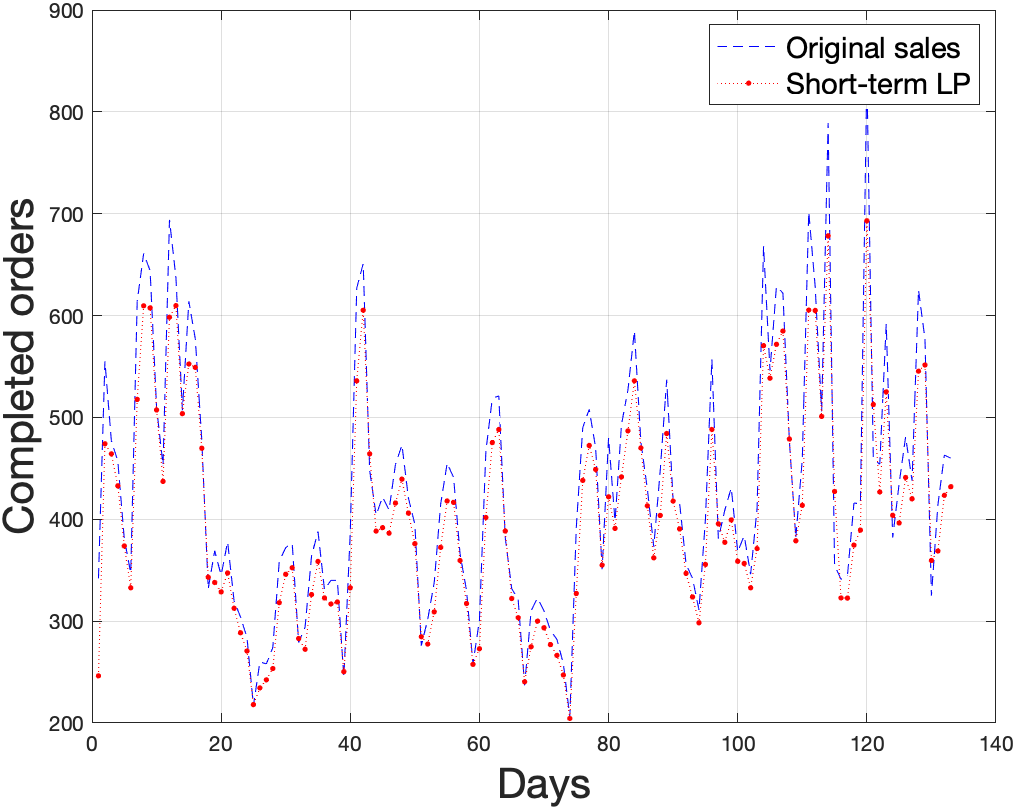
\includegraphics[width=\textwidth]{figures/expLP.png}
            \caption{Standard LP.}
            \label{fig:slpres}
        \end{subfigure}
        \hspace{0.1\textwidth}
        \begin{subfigure}[b]{0.4\textwidth}
            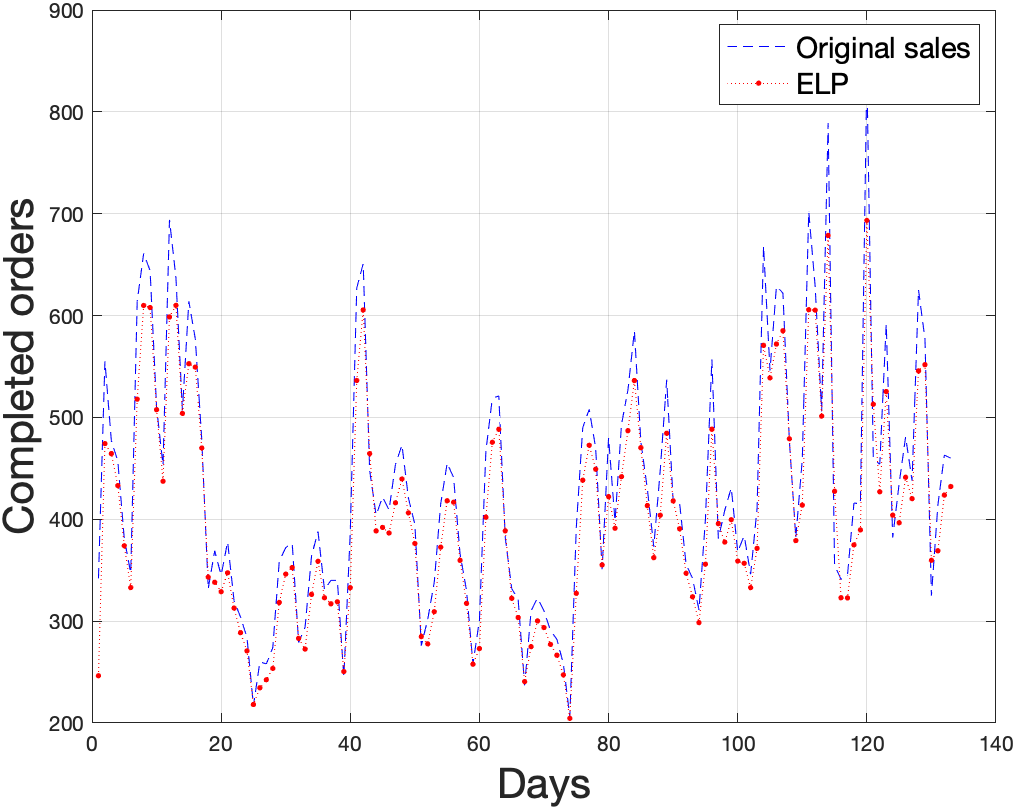
\includegraphics[width=\textwidth]{figures/expELP.png}
            \caption{Extended LP.}
            \label{fig:slpmse}
        \end{subfigure}
        \caption{Results of shot-term linear prediction.}
        \label{fig:shortresult}
    \end{figure}
    
    \subsubsection{Long-term linear prediction} \label{subsec:res_ltlp}
    ~an~R² value of 0.9160 means that 91.6\% of the~variation in the~dependent
    variable can be explained by the~independent variables in the~model.\\
    \\
    RMSE (Root Mean Square Error) and MSE (Mean Squared Error) are measures of the
    error or difference between the~actual values of the~dependent variable and the
    predicted values from the~model. RMSE is the~square root of the~average squared
    difference between the~predicted and actual values, while MSE is simply the
    average squared difference between them.\\
    \\
    In this case,~an~RMSE of 35.0163 means that on average, the~predicted values from
     the~model are about 35.02 units away from the~actual values. And the
    MSE of 1223.3 means that on average, the~squared difference between the~predicted
    and actual values is 1223.3. On figure \ref{fig:longresult} we can see predicted
    orders and on figure \ref{fig:ltlpmse} is the~prediction error for short-term
    linear prediction.
    \begin{figure}[h!]
        \centering
        \begin{subfigure}[b]{0.4\textwidth}
            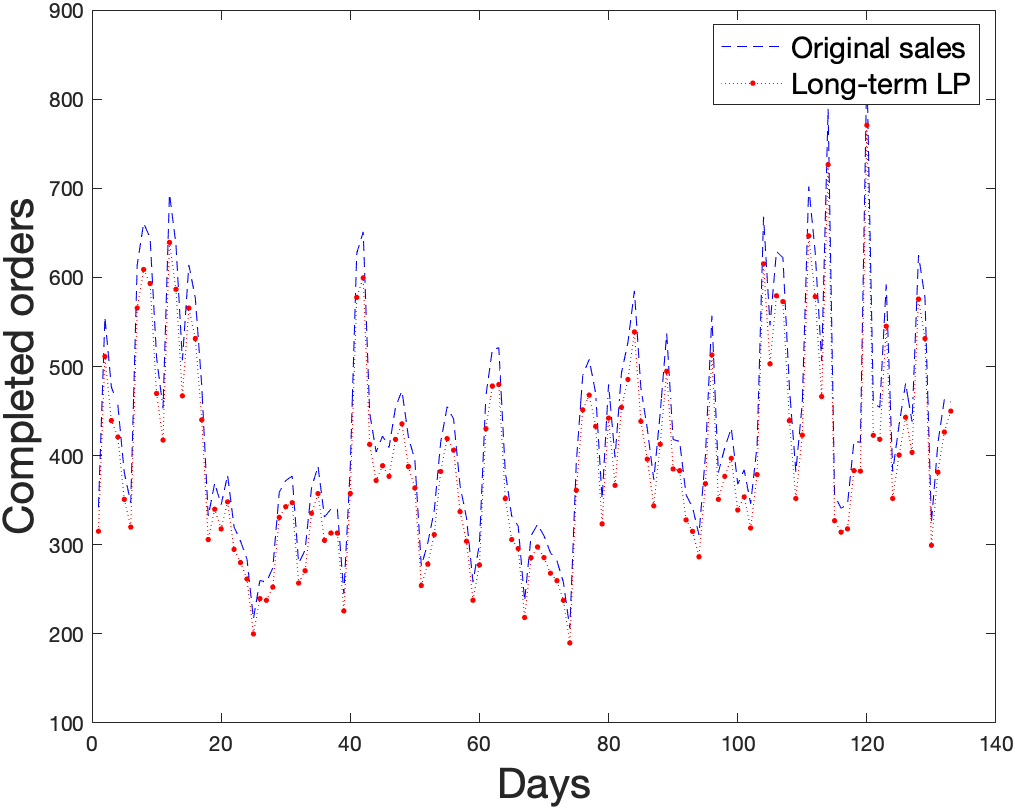
\includegraphics[width=1\textwidth]{figures/expLTLP.png}
            \caption{Standard LP.}
            \label{fig:ltlp}
        \end{subfigure}
        \hspace{0.1\textwidth}
        \begin{subfigure}[b]{0.4\textwidth}
            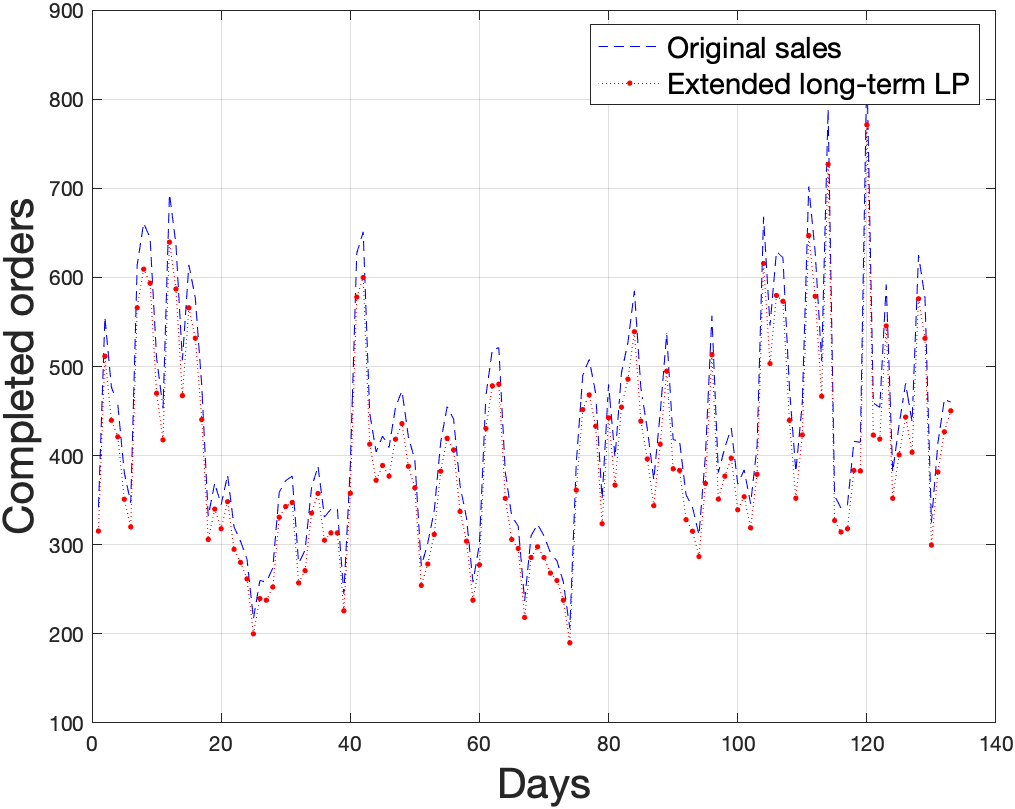
\includegraphics[width=1\textwidth]{figures/expELTLP.png}
            \caption{Extended LP.}
            \label{fig:eltlp}
        \end{subfigure}
        \caption{Results of long-term linear prediction.}
        \label{fig:longresult}
    \end{figure}
    
    \subsubsection{Extended long-term linear prediction} \label{subsec:res_eltlp}
     the~R-squared value of 0.9171 indicates that the~independent variables in the
    model can explain about 91.7\% of the~variation observed in the~dependent variable.
     the~RMSE and MSE are metrics used to evaluate the~accuracy of the~model's predictions
    compared to the~actual values. The~RMSE value of 34.7782 means that the~average difference
    between the~predicted and actual values is approximately 34.7 units. The~MSE value of
    1206.7 indicates that the~average squared difference between the~predicted and actual
    values is approximately 1206.7.\\
    \begin{figure}[!ht]
        \centering
        \begin{subfigure}[b]{0.4\textwidth}
            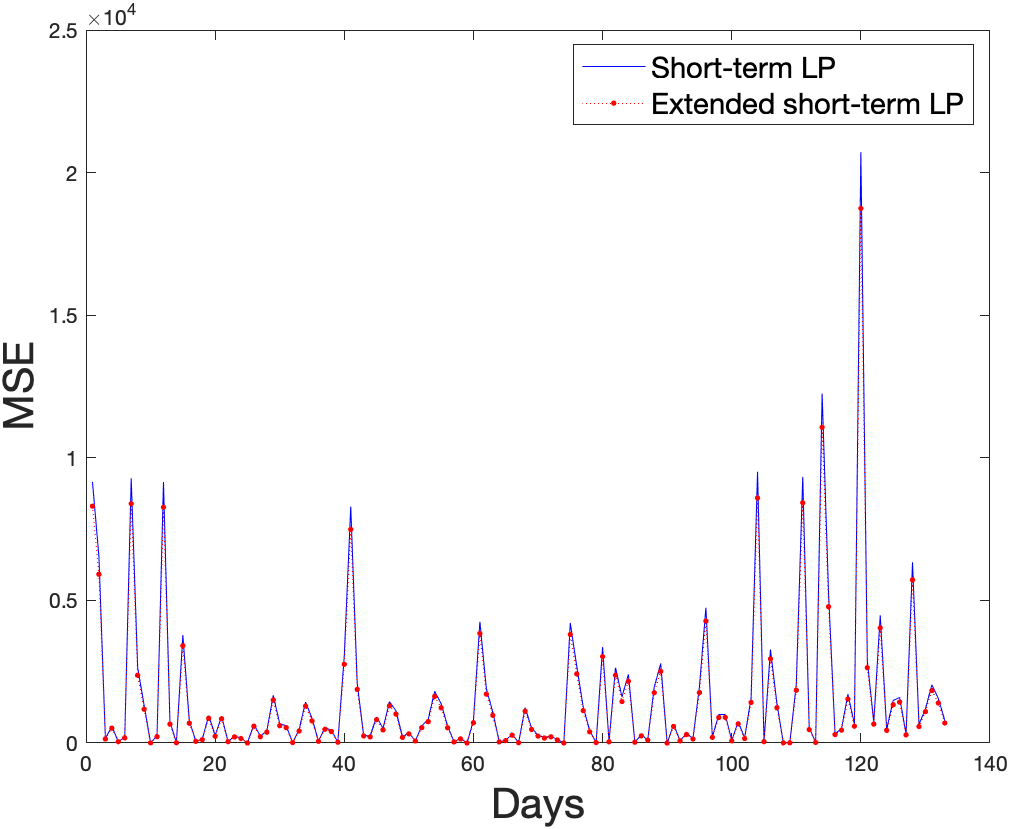
\includegraphics[width=1\textwidth]{figures/mseLP.png}
            \caption{Short-term LP.}
            \label{fig:mselp}
        \end{subfigure}
        \hspace{0.1\textwidth}
        \begin{subfigure}[b]{0.4\textwidth}
            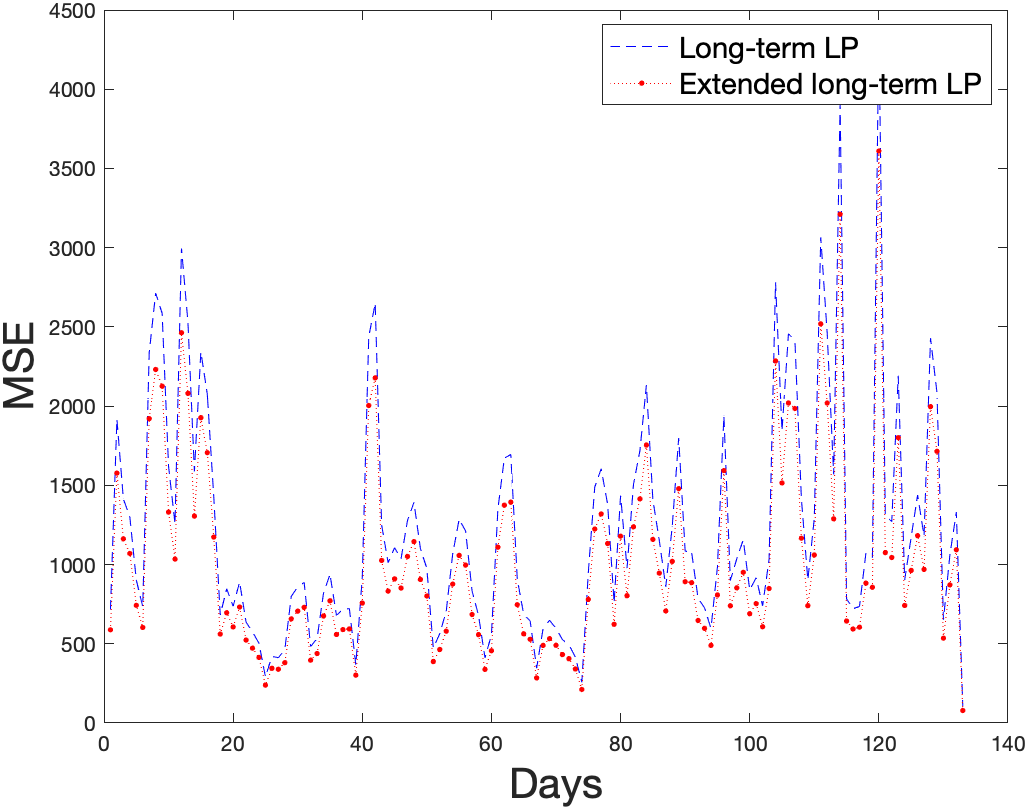
\includegraphics[width=1\textwidth]{figures/mseLLP.png}
            \caption{Long-term LP.}
            \label{fig:ltlpmse}
        \end{subfigure}
        \caption{Comparison of MSE for standard and extended LP.}
        \label{fig:mseresult}
    \end{figure}
    Overall, higher R-squared values and lower RMSE and MSE values in this model are
    desirable as they indicate a~better fit of the~model to the~data and better predictive accuracy.
    
    \subsubsection{Comparison of the~predictors} \label{subsec:res_comparison}
    Let's see results from our experiment in table \ref{tab:model_comparison} as we expected
    long term prediction is worst than long term prediction and apply extended weights to
    linear prediction made all comparison parameters better.\\
    \\
    On the~figures with MSE representation we can see the~main better point of long-term
    prediction for economical datasets. From $R^2$ and RMSE the~improvments of the~models is not
    see so higher than on the~figure \ref{fig:mseresults}.\\
    \newpage
    \begin{table}[!ht]
        \centering
        \begin{tabular}{|l|c|c|c|}
            \hline
            Model & $R^2$ & RMSE & MSE \\
            \hline
            Short-term linear prediction & 0.8872 & 40.6215 & 1650.1 \\
            Extended short-term linear prediction & 0.8881 & 40.4662 & 1637.5 \\
            Long-term linear prediction & 0.9160 & 35.0163 & 1223.3 \\
            Extended Long-term linear prediction & 0.9171 & 34.7782 & 1206.7 \\
            \hline
        \end{tabular}
        \caption{Comparison of linear prediction models}
        \label{tab:model_comparison}
    \end{table}

    \begin{figure}[h!]
        \centering
        \begin{subfigure}[b]{0.4\textwidth}
            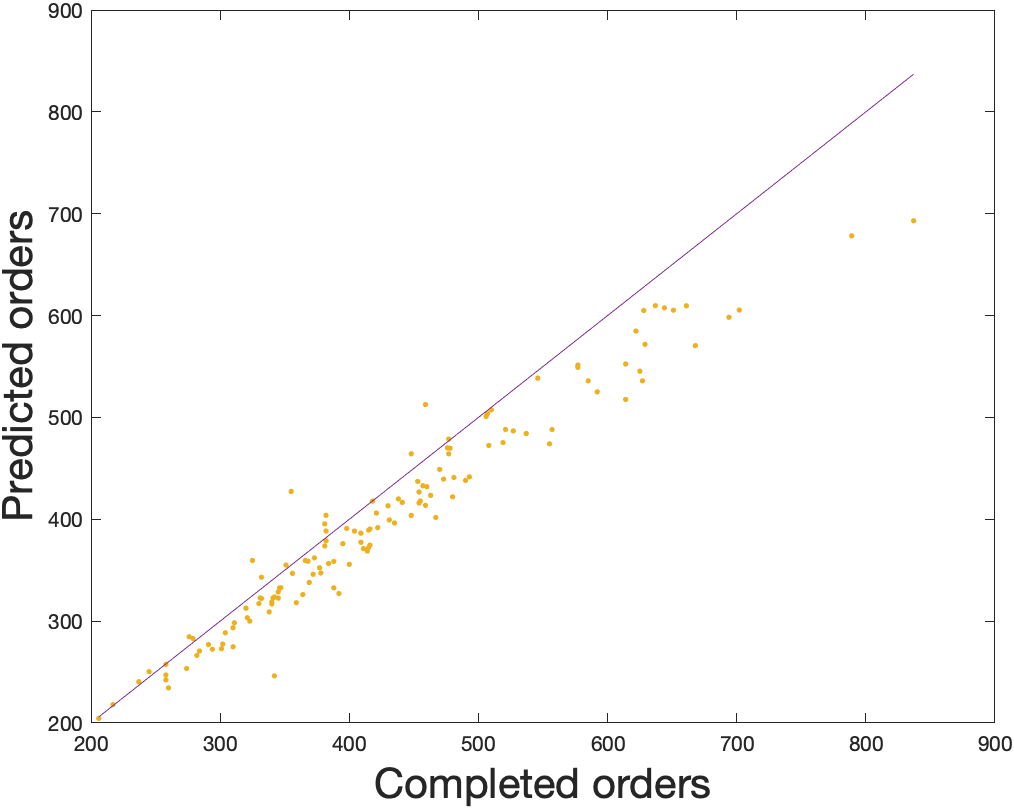
\includegraphics[width=\textwidth]{figures/expCompLP.png}
            \caption{Short-term linear prediction.}
            \label{fig:stlpres}
        \end{subfigure}
        \hspace{0.1\textwidth}
        \begin{subfigure}[b]{0.4\textwidth}
            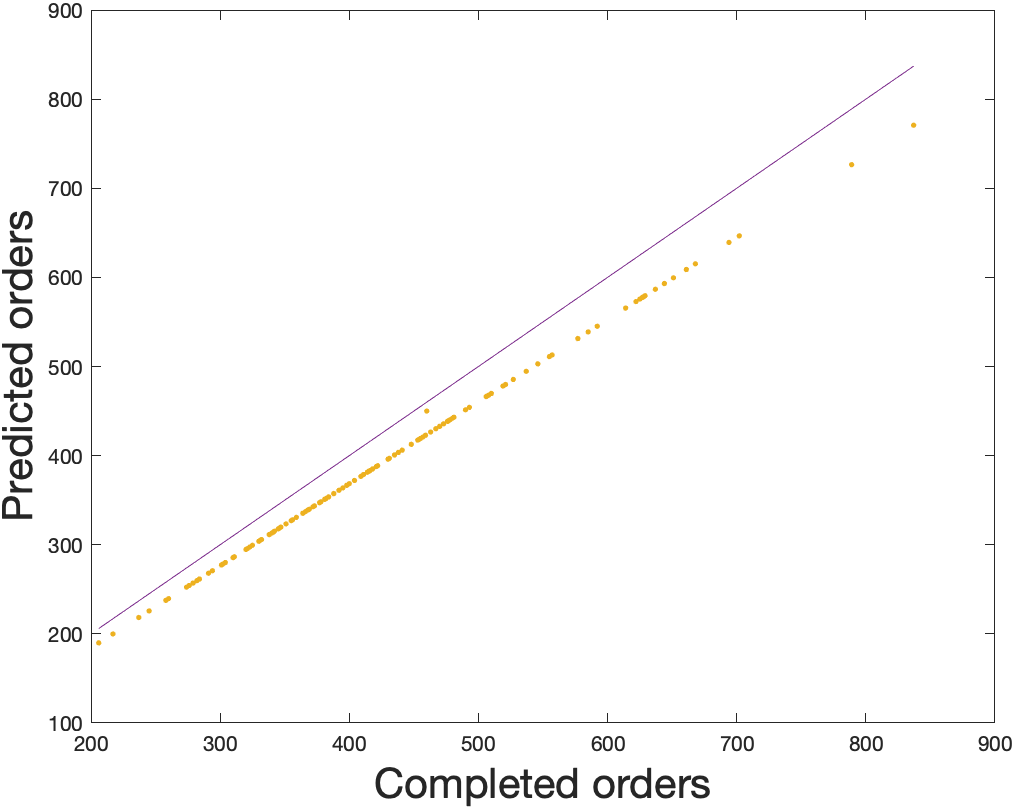
\includegraphics[width=\textwidth]{figures/expCompLTLP.png}
            \caption{Long-term linear prediction.}
            \label{fig:eltlpres}
        \end{subfigure}
        \begin{subfigure}[b]{0.4\textwidth}
            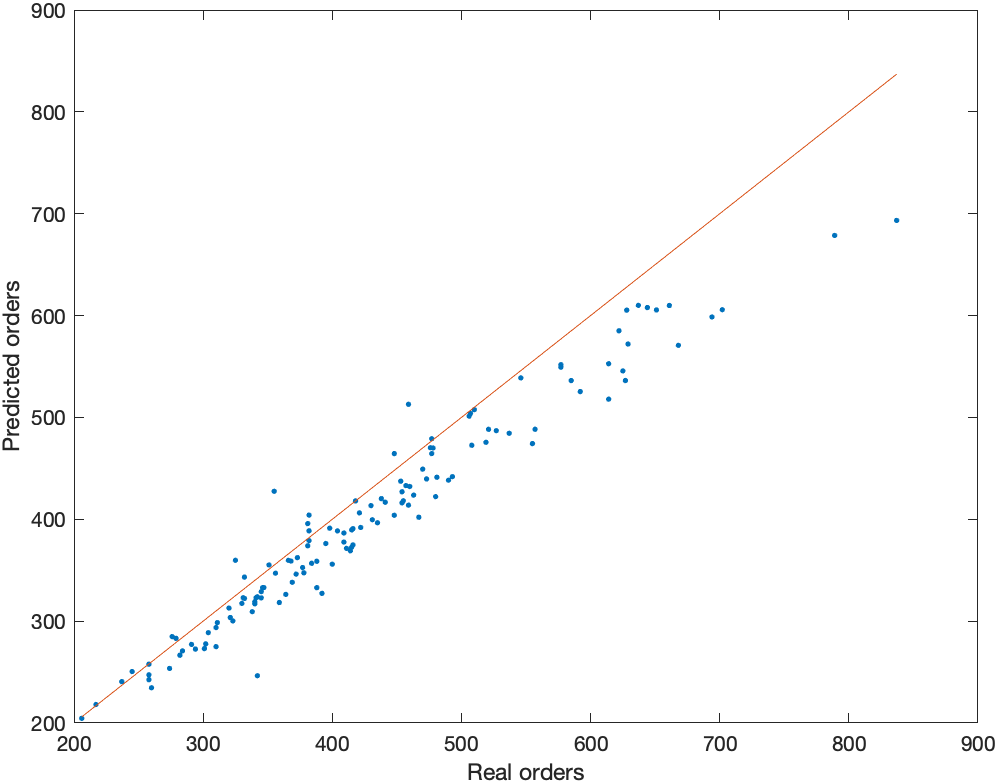
\includegraphics[width=\textwidth]{figures/expCompELP.png}
            \caption{Extended short-term LP.}
            \label{fig:eslpmse}
        \end{subfigure}
        \hspace{0.1\textwidth}
        \begin{subfigure}[b]{0.4\textwidth}
            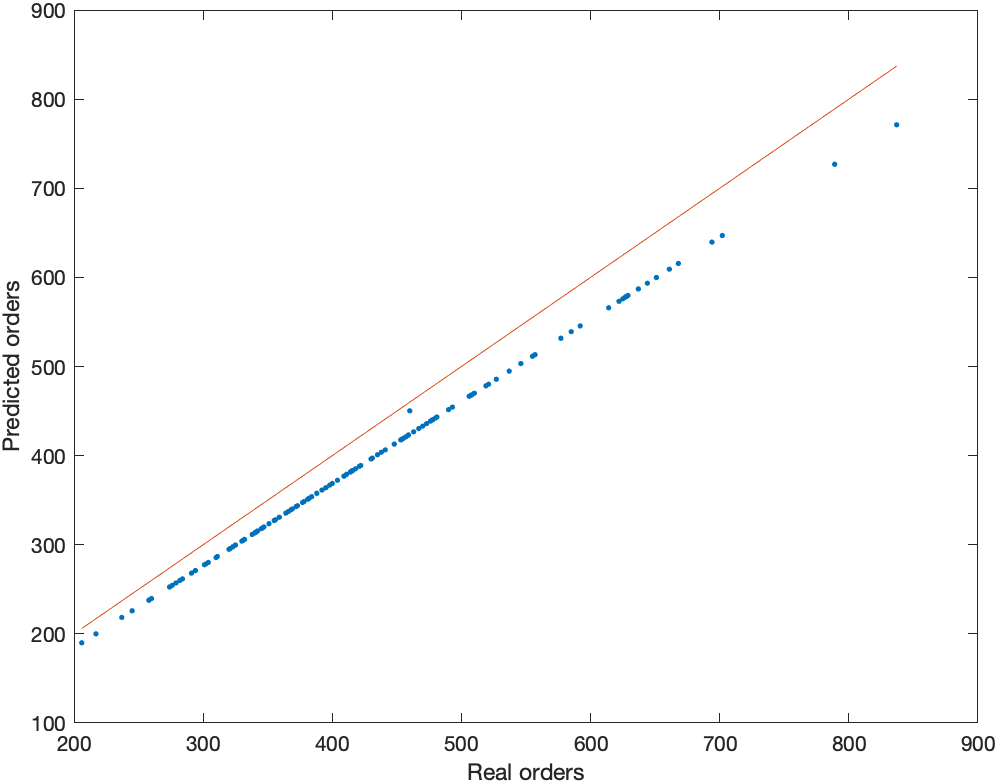
\includegraphics[width=\textwidth]{figures/expCompELTLP.png}
            \caption{Extended long-term LP.}
            \label{fig:eltlpmse}
        \end{subfigure}
        \caption{Results of prediction performance.}
        \label{fig:mseresults}
    \end{figure}
    
    On the figure~\ref{fig:mseresults} we can see the main results and
    differences between the models. We can see the less variance in
    long-term predictors (figures \ref{fig:eltlpres}, \ref{fig:eltlpmse})
    than in short one (figures \ref{fig:stlpres}, \ref{fig:eslpmse}).
